% Options for packages loaded elsewhere
\PassOptionsToPackage{unicode}{hyperref}
\PassOptionsToPackage{hyphens}{url}
%
\documentclass[
]{book}
\usepackage{lmodern}
\usepackage{amssymb,amsmath}
\usepackage{ifxetex,ifluatex}
\ifnum 0\ifxetex 1\fi\ifluatex 1\fi=0 % if pdftex
  \usepackage[T1]{fontenc}
  \usepackage[utf8]{inputenc}
  \usepackage{textcomp} % provide euro and other symbols
\else % if luatex or xetex
  \usepackage{unicode-math}
  \defaultfontfeatures{Scale=MatchLowercase}
  \defaultfontfeatures[\rmfamily]{Ligatures=TeX,Scale=1}
\fi
% Use upquote if available, for straight quotes in verbatim environments
\IfFileExists{upquote.sty}{\usepackage{upquote}}{}
\IfFileExists{microtype.sty}{% use microtype if available
  \usepackage[]{microtype}
  \UseMicrotypeSet[protrusion]{basicmath} % disable protrusion for tt fonts
}{}
\makeatletter
\@ifundefined{KOMAClassName}{% if non-KOMA class
  \IfFileExists{parskip.sty}{%
    \usepackage{parskip}
  }{% else
    \setlength{\parindent}{0pt}
    \setlength{\parskip}{6pt plus 2pt minus 1pt}}
}{% if KOMA class
  \KOMAoptions{parskip=half}}
\makeatother
\usepackage{xcolor}
\IfFileExists{xurl.sty}{\usepackage{xurl}}{} % add URL line breaks if available
\IfFileExists{bookmark.sty}{\usepackage{bookmark}}{\usepackage{hyperref}}
\hypersetup{
  pdftitle={Drone Guides},
  hidelinks,
  pdfcreator={LaTeX via pandoc}}
\urlstyle{same} % disable monospaced font for URLs
\usepackage{color}
\usepackage{fancyvrb}
\newcommand{\VerbBar}{|}
\newcommand{\VERB}{\Verb[commandchars=\\\{\}]}
\DefineVerbatimEnvironment{Highlighting}{Verbatim}{commandchars=\\\{\}}
% Add ',fontsize=\small' for more characters per line
\usepackage{framed}
\definecolor{shadecolor}{RGB}{248,248,248}
\newenvironment{Shaded}{\begin{snugshade}}{\end{snugshade}}
\newcommand{\AlertTok}[1]{\textcolor[rgb]{0.94,0.16,0.16}{#1}}
\newcommand{\AnnotationTok}[1]{\textcolor[rgb]{0.56,0.35,0.01}{\textbf{\textit{#1}}}}
\newcommand{\AttributeTok}[1]{\textcolor[rgb]{0.77,0.63,0.00}{#1}}
\newcommand{\BaseNTok}[1]{\textcolor[rgb]{0.00,0.00,0.81}{#1}}
\newcommand{\BuiltInTok}[1]{#1}
\newcommand{\CharTok}[1]{\textcolor[rgb]{0.31,0.60,0.02}{#1}}
\newcommand{\CommentTok}[1]{\textcolor[rgb]{0.56,0.35,0.01}{\textit{#1}}}
\newcommand{\CommentVarTok}[1]{\textcolor[rgb]{0.56,0.35,0.01}{\textbf{\textit{#1}}}}
\newcommand{\ConstantTok}[1]{\textcolor[rgb]{0.00,0.00,0.00}{#1}}
\newcommand{\ControlFlowTok}[1]{\textcolor[rgb]{0.13,0.29,0.53}{\textbf{#1}}}
\newcommand{\DataTypeTok}[1]{\textcolor[rgb]{0.13,0.29,0.53}{#1}}
\newcommand{\DecValTok}[1]{\textcolor[rgb]{0.00,0.00,0.81}{#1}}
\newcommand{\DocumentationTok}[1]{\textcolor[rgb]{0.56,0.35,0.01}{\textbf{\textit{#1}}}}
\newcommand{\ErrorTok}[1]{\textcolor[rgb]{0.64,0.00,0.00}{\textbf{#1}}}
\newcommand{\ExtensionTok}[1]{#1}
\newcommand{\FloatTok}[1]{\textcolor[rgb]{0.00,0.00,0.81}{#1}}
\newcommand{\FunctionTok}[1]{\textcolor[rgb]{0.00,0.00,0.00}{#1}}
\newcommand{\ImportTok}[1]{#1}
\newcommand{\InformationTok}[1]{\textcolor[rgb]{0.56,0.35,0.01}{\textbf{\textit{#1}}}}
\newcommand{\KeywordTok}[1]{\textcolor[rgb]{0.13,0.29,0.53}{\textbf{#1}}}
\newcommand{\NormalTok}[1]{#1}
\newcommand{\OperatorTok}[1]{\textcolor[rgb]{0.81,0.36,0.00}{\textbf{#1}}}
\newcommand{\OtherTok}[1]{\textcolor[rgb]{0.56,0.35,0.01}{#1}}
\newcommand{\PreprocessorTok}[1]{\textcolor[rgb]{0.56,0.35,0.01}{\textit{#1}}}
\newcommand{\RegionMarkerTok}[1]{#1}
\newcommand{\SpecialCharTok}[1]{\textcolor[rgb]{0.00,0.00,0.00}{#1}}
\newcommand{\SpecialStringTok}[1]{\textcolor[rgb]{0.31,0.60,0.02}{#1}}
\newcommand{\StringTok}[1]{\textcolor[rgb]{0.31,0.60,0.02}{#1}}
\newcommand{\VariableTok}[1]{\textcolor[rgb]{0.00,0.00,0.00}{#1}}
\newcommand{\VerbatimStringTok}[1]{\textcolor[rgb]{0.31,0.60,0.02}{#1}}
\newcommand{\WarningTok}[1]{\textcolor[rgb]{0.56,0.35,0.01}{\textbf{\textit{#1}}}}
\usepackage{longtable,booktabs}
% Correct order of tables after \paragraph or \subparagraph
\usepackage{etoolbox}
\makeatletter
\patchcmd\longtable{\par}{\if@noskipsec\mbox{}\fi\par}{}{}
\makeatother
% Allow footnotes in longtable head/foot
\IfFileExists{footnotehyper.sty}{\usepackage{footnotehyper}}{\usepackage{footnote}}
\makesavenoteenv{longtable}
\usepackage{graphicx,grffile}
\makeatletter
\def\maxwidth{\ifdim\Gin@nat@width>\linewidth\linewidth\else\Gin@nat@width\fi}
\def\maxheight{\ifdim\Gin@nat@height>\textheight\textheight\else\Gin@nat@height\fi}
\makeatother
% Scale images if necessary, so that they will not overflow the page
% margins by default, and it is still possible to overwrite the defaults
% using explicit options in \includegraphics[width, height, ...]{}
\setkeys{Gin}{width=\maxwidth,height=\maxheight,keepaspectratio}
% Set default figure placement to htbp
\makeatletter
\def\fps@figure{htbp}
\makeatother
\setlength{\emergencystretch}{3em} % prevent overfull lines
\providecommand{\tightlist}{%
  \setlength{\itemsep}{0pt}\setlength{\parskip}{0pt}}
\setcounter{secnumdepth}{5}
\usepackage{booktabs}
\usepackage[]{natbib}
\bibliographystyle{apalike}

\title{Drone Guides}
\author{}
\date{\vspace{-2.5em}}

\begin{document}
\maketitle

{
\setcounter{tocdepth}{1}
\tableofcontents
}
\begin{Shaded}
\begin{Highlighting}[]
\NormalTok{foo <-}\StringTok{ }\ControlFlowTok{function}\NormalTok{(x)\{}
  \ControlFlowTok{for}\NormalTok{( i }\ControlFlowTok{in}\NormalTok{ x )\{}
    \CommentTok{#  require returns TRUE invisibly if it was able to load package}
    \ControlFlowTok{if}\NormalTok{( }\OperatorTok{!}\StringTok{ }\KeywordTok{require}\NormalTok{( i , }\DataTypeTok{character.only =} \OtherTok{TRUE}\NormalTok{ ) )\{}
      \CommentTok{#  If package was not able to be loaded then re-install}
      \KeywordTok{install.packages}\NormalTok{( i , }\DataTypeTok{dependencies =} \OtherTok{TRUE}\NormalTok{ )}
      \CommentTok{#  Load package after installing}
      \KeywordTok{require}\NormalTok{( i , }\DataTypeTok{character.only =} \OtherTok{TRUE}\NormalTok{ )}
\NormalTok{    \}}
\NormalTok{  \}}
\NormalTok{\}}

\CommentTok{#  Then try/install packages...}
\KeywordTok{foo}\NormalTok{( }\KeywordTok{c}\NormalTok{(}\StringTok{"bookdown"}\NormalTok{ , }\StringTok{"DiagrammeR"}\NormalTok{ ) )}
\end{Highlighting}
\end{Shaded}

\hypertarget{ch-getting-started}{%
\chapter{Drone Guide Portal}\label{ch-getting-started}}

\begin{center}
\includegraphics[width=0.5\linewidth]{images/COE_logo} \end{center}

In this portal, you'll find links to various tutorials and guides for drone users of all levels.

This page will be a work in progress and new resources will be added periodically. Feel free to reach out to us at \href{mailto:UASSafety@ucmerced.edu}{\nolinkurl{UASSafety@ucmerced.edu}} if you have any questions or would like to see additional resources added.

If you're interested in contributing a tutorial or guide, please feel free to fork this repository and add your content. This guide is developed in RStudio using bookdown. All content is generated from the markdown files in the main directory.

\hypertarget{ch-camera-settings}{%
\chapter{How to Set Your Settings For Good Media Cinematography}\label{ch-camera-settings}}

\hypertarget{uc-center-of-excellence-on-unmanned-aircraft-system-safety}{%
\section{UC Center of Excellence on Unmanned Aircraft System Safety}\label{uc-center-of-excellence-on-unmanned-aircraft-system-safety}}

\hypertarget{rule-one-understand-the-settings-within-a-drone}{%
\paragraph{Rule one: Understand The Settings within a Drone}\label{rule-one-understand-the-settings-within-a-drone}}

** Below is a break down of the settings base on this image **

\hypertarget{camera-settings}{%
\subsection{Camera Settings}\label{camera-settings}}

\begin{itemize}
\tightlist
\item
  ISO
\item
  Shutter Speed
\item
  Aperature
  \#\#\# Photo Settings
\item
  Single Shot
\item
  HDR Shot
\item
  Multiple
\item
  AEB
\item
  Timed Shot
\item
  Pano
\item
  ShallowFocus
  \#\#\# Other Settings
\item
  Image Size
\item
  Image Format
\item
  White Balance
\item
  Style
\item
  Color
\end{itemize}

\hypertarget{camera-settings-1}{%
\chapter{Camera Settings}\label{camera-settings-1}}

\hypertarget{iso}{%
\subsection{Iso}\label{iso}}

ISO measures the sensitivity of the image sensor. The lower the number the less sensitive your camera is to light and the finer the grain. By choosing a higher ISO you can use a faster shutter speed to freeze the movement. Higher numbers mean your sensor becomes more sensitive to light which allows you to use your camera in darker situations, but the cost of doing so is more grain.

\hypertarget{shutter-speed}{%
\subsection{Shutter Speed}\label{shutter-speed}}

The Shutter controls for how long light is let into the lenses. To simplify the shutter, a low shutter speed lets more light in and is good for taking pictures in dim lighting while a high shutter speed lets in more light and is good for taking crisp shots of moving objects or people. In S mode, you can set the shutter speed, but other settings will be set automatically to match exposure.

\hypertarget{aperature}{%
\subsection{Aperature}\label{aperature}}

This controls how much light gets through when you take a picture. This is measured in `f-stops.' A smaller f-stop number means a bigger aperture and so more light comes through, and a bigger f-stop number means a smaller aperture, so less light comes through. In A mode, you can set the Aperture, but other settings will still be set automatically to match exposure.

\begin{verbatim}
## NULL
\end{verbatim}

\hypertarget{photo-settings}{%
\chapter{Photo Settings}\label{photo-settings}}

\hypertarget{single-shot}{%
\subsection{Single Shot}\label{single-shot}}

The standard mode, it takes a 1 picture every time you tap the shoot button.
\#\#\# HDR Shot
The camera will take three images of the same scene. One will be underexposed, another overexposed and the last will be properly exposed then it will combine the three images to create a more dynamic JPEG.

\hypertarget{multiple}{%
\subsection{Multiple}\label{multiple}}

With this mode, the camera will take multiple pictures when you press the shoot button. You might want to use this mode if you are trying to get a shot of a moving subject.

\hypertarget{aeb-automatic-exposure-bracketing}{%
\subsection{AEB (Automatic Exposure Bracketing)}\label{aeb-automatic-exposure-bracketing}}

A set of 3 or 5 shots that work similarly to HDR Shots taking overexposed, underexposed and properly exposed photos. However, in AEB the images are in RAW and they are not combine.

\hypertarget{timed-shot}{%
\subsection{Timed Shot}\label{timed-shot}}

This allows you to set a countdown timer before the shot is taken, it's useful for taking selfies.

\hypertarget{pano}{%
\subsection{Pano}\label{pano}}

180° Panorama mode can stitch 21 photos together to create a 180° panoramic photo.

\begin{verbatim}
## NULL
\end{verbatim}

\hypertarget{shallowfocus}{%
\subsection{ShallowFocus}\label{shallowfocus}}

This mode allows you to create a depth of field effect in your photo.

\hypertarget{other-settings}{%
\chapter{Other Settings}\label{other-settings}}

\hypertarget{image-size}{%
\subsection{Image Size}\label{image-size}}

You can choose the size of your picture 4:3,16:9 3:2. 4:3 was the old standard 33mm size. 16:9 is the common size for HD capable devices and 3:2 is the traditional size for printed photos.
\#\#\# Image Format
In this area, you can choose between taking photos in RAW, JPEG and RAW + JPEG. Raw is a file format that captures all image data recorded by the sensor when you take a photo. JPEG a format for compressing image files.
\#\#\# White Balance
This is the process of removing unrealistic color casts so that objects which appear white in person are rendered white in your photo. It is measured in Kelvins. If you have Auto selected, then the camera will decide what the best setting is. You can also choose from a selection of profiles or set it yourself. Kelvin Temperature is simply a unit of measurement for temperature and in photography we most often use it to measure the color temperature of light sources. The temperature scale most often used in photography ranges from about 2000K (K=Kelvin) to 9000K.

\begin{verbatim}
## NULL
\end{verbatim}

\hypertarget{style}{%
\subsection{Style}\label{style}}

This is where you can configure the sharpness, contrast, and saturation of the images or videos that your drone's camera takes. (Triangle) Digital Sharpness this makes the picture sharper. (Circle) Contrast controls the strength of the lights and the darks in the picture. (Rectangle) Saturation of colors low saturation makes the photos look dull, and high saturation make the colors pop. These can be set in a range of -3 to +3.
\#\#\# Color
Here you can set the camera color profile. These settings affect the colors in your photo. D -- Cinelike and D --Log are both designed for taking photos that will be post-processed later on. The rest of the color profiles are ready to go with no post-processing required.

\hypertarget{rule-two-make-sure-your-settings-are-a-lined-with-the-weather}{%
\section{Rule two: Make sure your settings are a lined with the Weather}\label{rule-two-make-sure-your-settings-are-a-lined-with-the-weather}}

\hypertarget{cloudy-and-overcast-days}{%
\subsection{Cloudy and Overcast Days}\label{cloudy-and-overcast-days}}

A cloudy and Overcast day gives an amazing amount of diffused light. You can also shoot in the middle of the day with little worry about harsh lighting or unwanted shadows. Theres a catch though when shooting scenary feel in overcast conditions can also be challenging. Overcast skies are gray and don't usually add a lot of interest to that mountainscape, or field of cows you want to photograph. Look for stormy weather clouds, that add a sense of place and dimension. You can also crop your shot so that you don't get those unwanted gray skies, but still get great lighting. This means you will be shooting with the lower side of the settings like lower aperature, ISO, and Shutter Speed.

\hypertarget{sunny-days}{%
\subsection{Sunny Days}\label{sunny-days}}

Landscapes in bright sun are absolutely beautiful. Try shooting the beach in the full sun of the day usually around 1 or 2pm. Practice exposing for the beautiful blue skies as well as the sand. Make sure you have high aperature, ISO, and Shutterspeed to keep your shots from being over exposed. Of course this is always mannual correction when editing, but you want to take photos that need little to none editing when shooting.

\hypertarget{rule-3-make-sure-you-always-double-check-your-shots-after-shooting}{%
\subsection{Rule 3: Make Sure you always double check your shots after shooting}\label{rule-3-make-sure-you-always-double-check-your-shots-after-shooting}}

Make sure you are always going back to shots and making sure they what you had in mind with the settings and the feel you are going for. You do not want to take a shot and then just think it was good enough, I always like to have about 4-6 shots with different settings and different feels. The reason being is that its always better to have opitions, because sometimes what you get out and about does not look the same when your uploading.

\hypertarget{ch-uas-settings.Rmd}{%
\chapter{General UAS Settings}\label{ch-uas-settings.Rmd}}

\hypertarget{main-control-mc-settings}{%
\section{Main Control (MC) Settings}\label{main-control-mc-settings}}

\begin{figure}
\centering
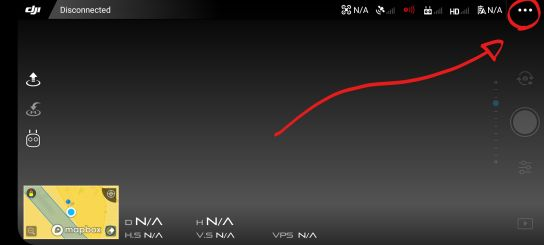
\includegraphics{images/DJI-SettingsPage.jpg}
\caption{Arrow indicating settings page location}
\end{figure}

The main control settings tab allows the user to modify a number of basic settings such as

\begin{figure}
\centering
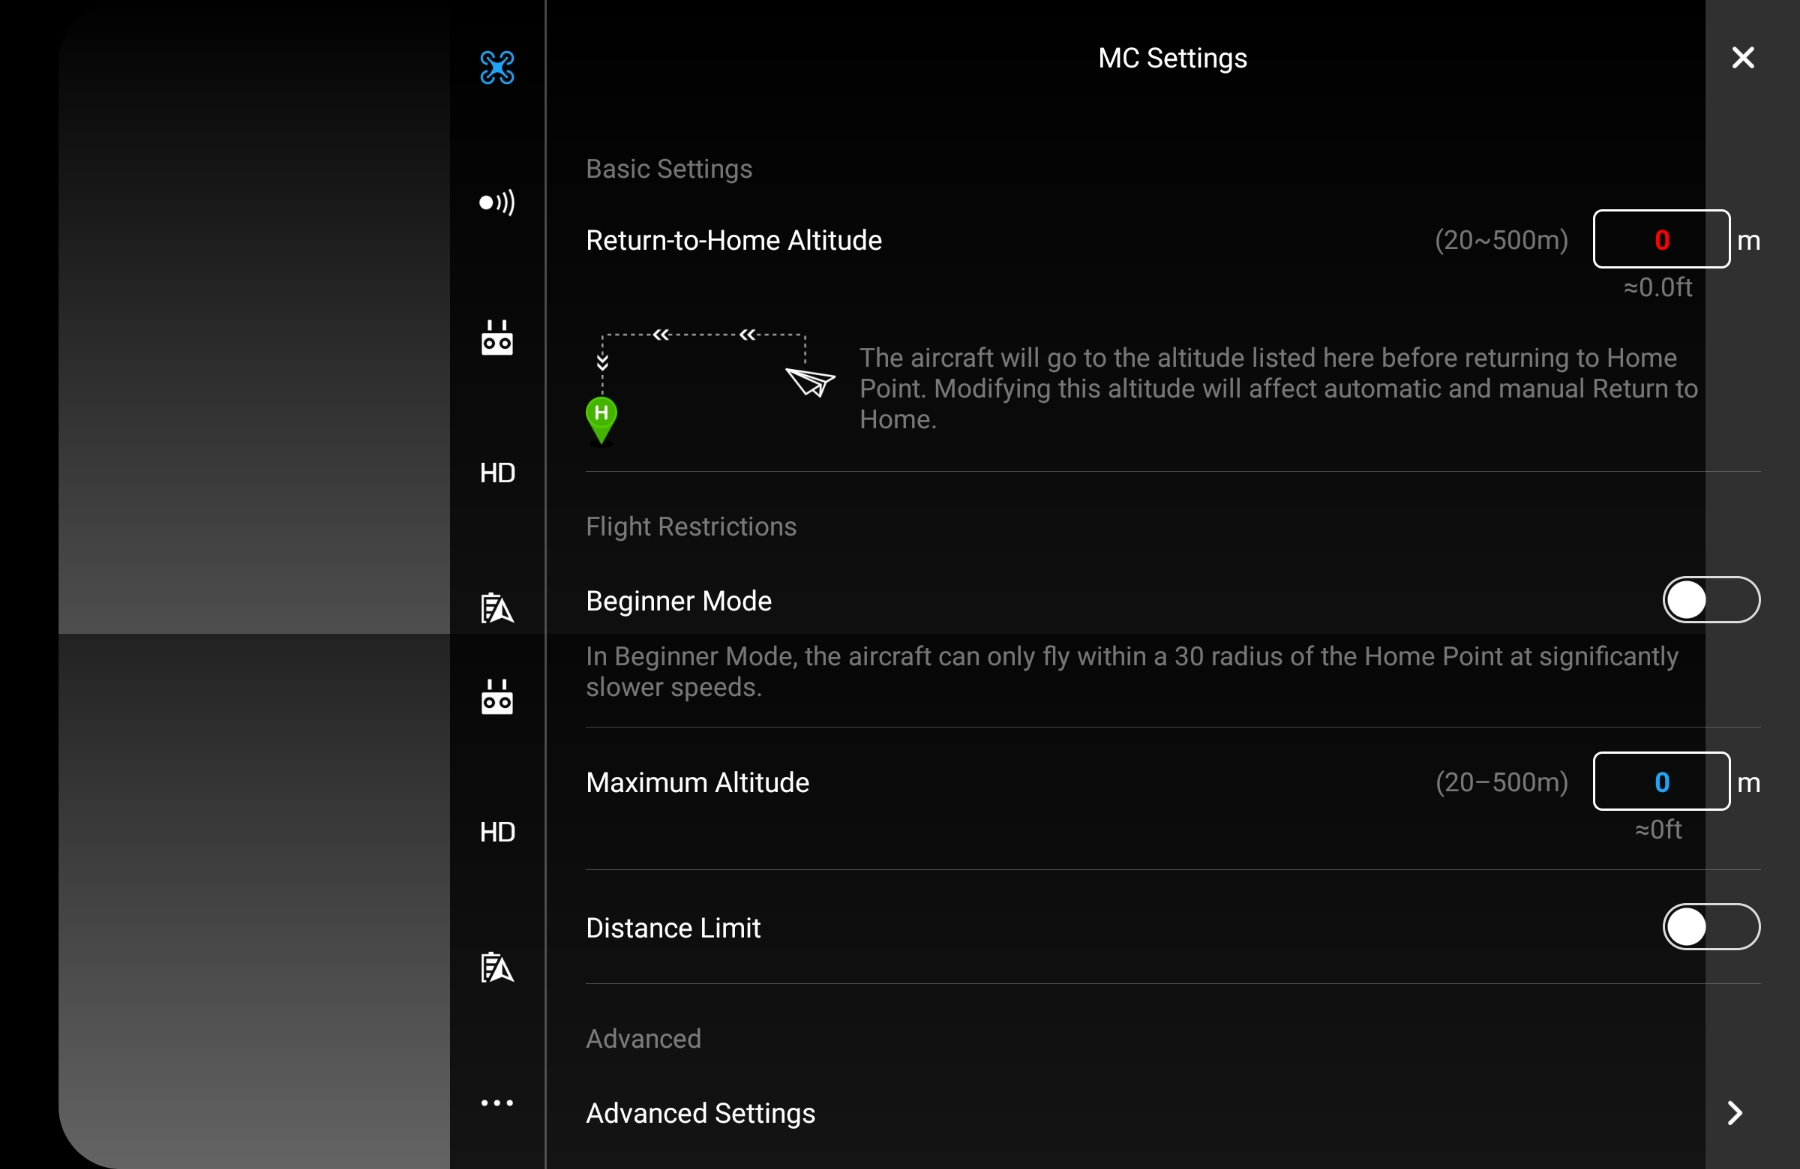
\includegraphics{images/MC/DJI-MC-SettingsPage.jpg}
\caption{Main Control Settings}
\end{figure}

\begin{enumerate}
\def\labelenumi{\arabic{enumi}.}
\tightlist
\item
  Return-to-Home Altitude
\item
  Beginner Mode
\item
  Maximum Altitude
\item
  Distance Limit
\end{enumerate}

with more advanced settings found at the bottom of the page.

\hypertarget{advanced-settings}{%
\subsection{Advanced Settings}\label{advanced-settings}}

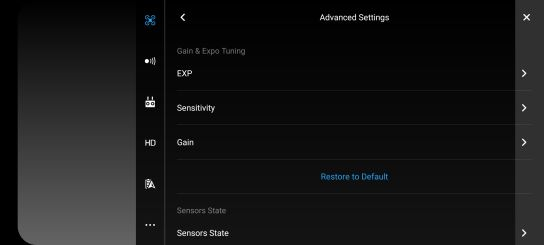
\includegraphics{images/MC/DJI-MC-Advanced-Settings.jpg}
The Advanced Settings page allows us access to a few different aircraft sensitivity settings.

\begin{enumerate}
\def\labelenumi{\arabic{enumi}.}
\tightlist
\item
  EXP
\end{enumerate}

\begin{figure}
\centering
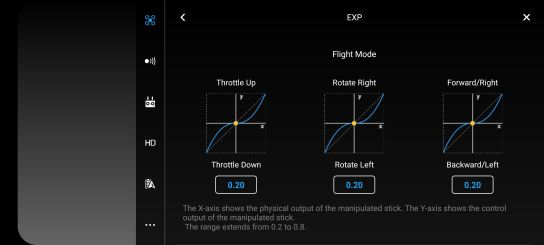
\includegraphics{images/MC/DJI-ExpSettings.jpg}
\caption{EXP settings}
\end{figure}

Tuning the EXP settings allows you to increase/decrease stick input sensitivity. The X-axis indicates user stick input and the Y-axis represents the ``value'' being output to the motors from these stick inputs. The higher the value, the more sensitive the drone can be towards the input stick movement. This is not to be confused with the next setting below.

\begin{enumerate}
\def\labelenumi{\arabic{enumi}.}
\setcounter{enumi}{1}
\tightlist
\item
  Sensitivity
\end{enumerate}

\begin{figure}
\centering
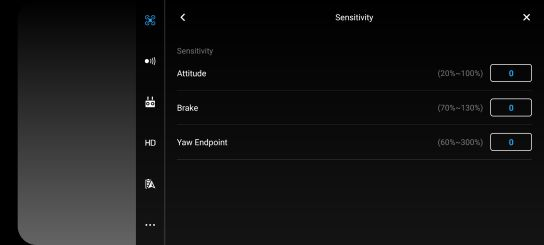
\includegraphics{images/MC/DJI-SensitivitySettings.jpg}
\caption{Sensitivity settings}
\end{figure}

The sensitivity setting affects how rapidly the drone will respond to the input. A higher value would cause the drone to react more aggressively while a lower value would dull out that same input.

\begin{enumerate}
\def\labelenumi{\arabic{enumi}.}
\setcounter{enumi}{2}
\tightlist
\item
  Gain
\end{enumerate}

\begin{figure}
\centering
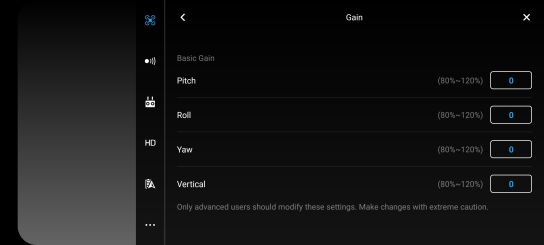
\includegraphics{images/MC/DJI-GainSettings.jpg}
\caption{Gain settings}
\end{figure}

Generally, the gain settingss are left alone.

\emph{General comment for myself, try and get a drone to checkout some of these functions before you can specifically state what it is that they do. There are some contradicting pieces of information found on the ``Gain'' settings and I don't want to give the wrong words of advice for something that can be sensitive to errors.}

\hypertarget{visual-navigation-settings}{%
\section{Visual Navigation Settings}\label{visual-navigation-settings}}

\begin{figure}
\centering
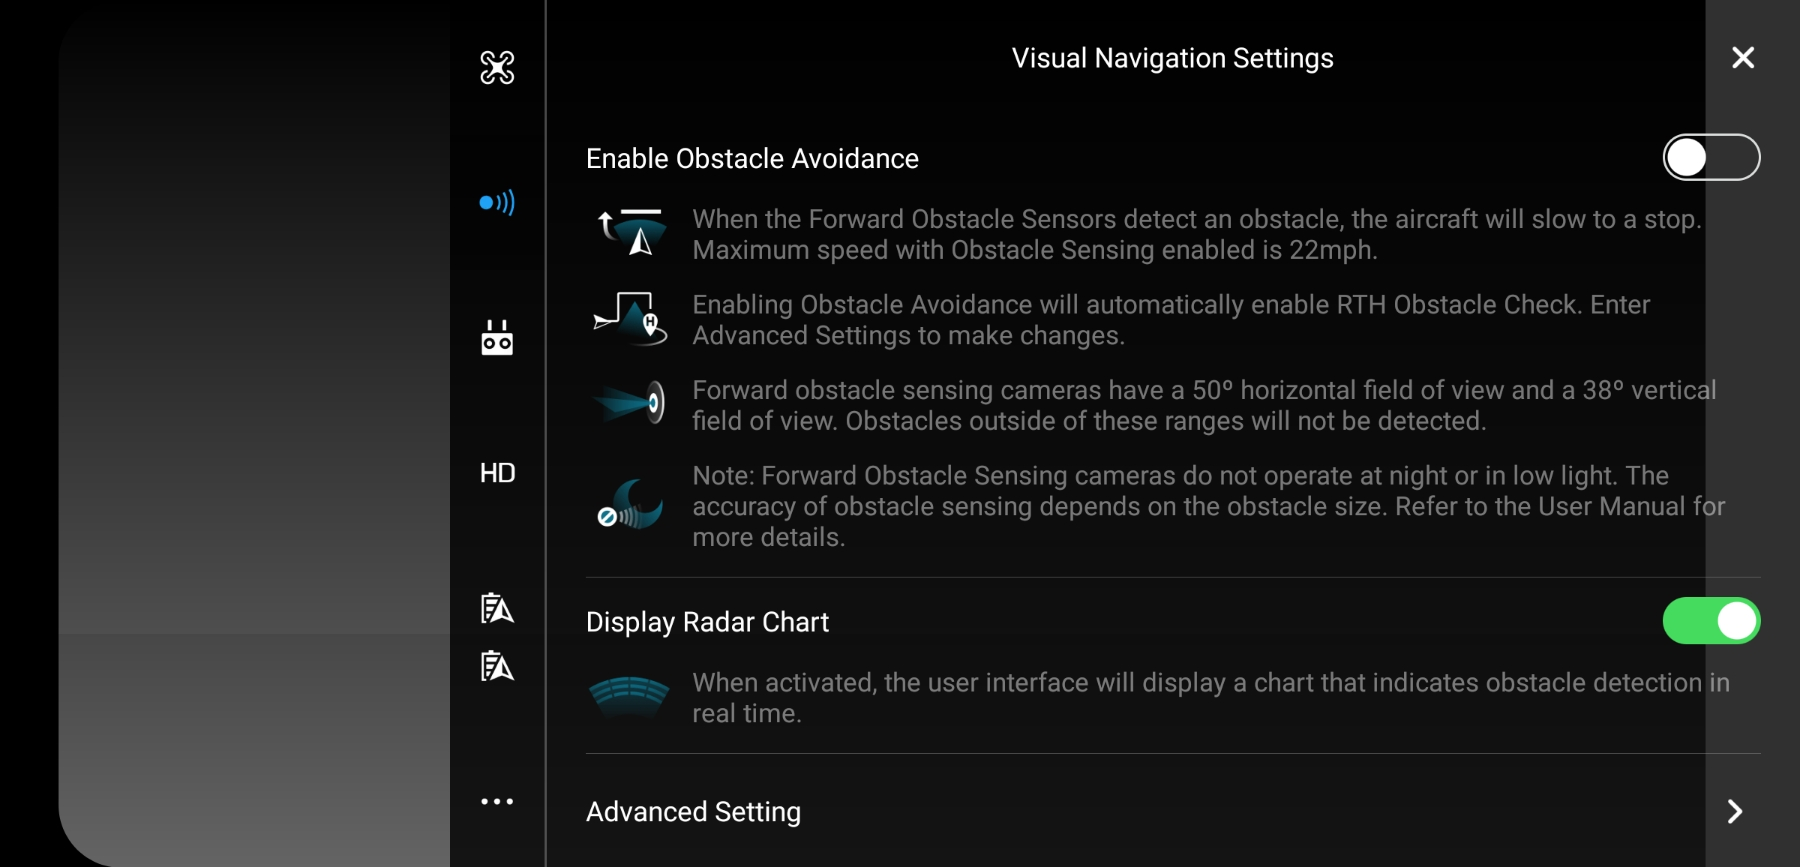
\includegraphics{images/VN/DJI-VisualNavigationSettings.jpg}
\caption{Visual Navigation Settings Page}
\end{figure}

Here we can toggle the Obstacle avoidance on and off, as well as the Radar Chart that displays real time obstacle detection. At the bottom we can again find Advanced Settings that pertain to the systems Visual navigation.

\begin{figure}
\centering
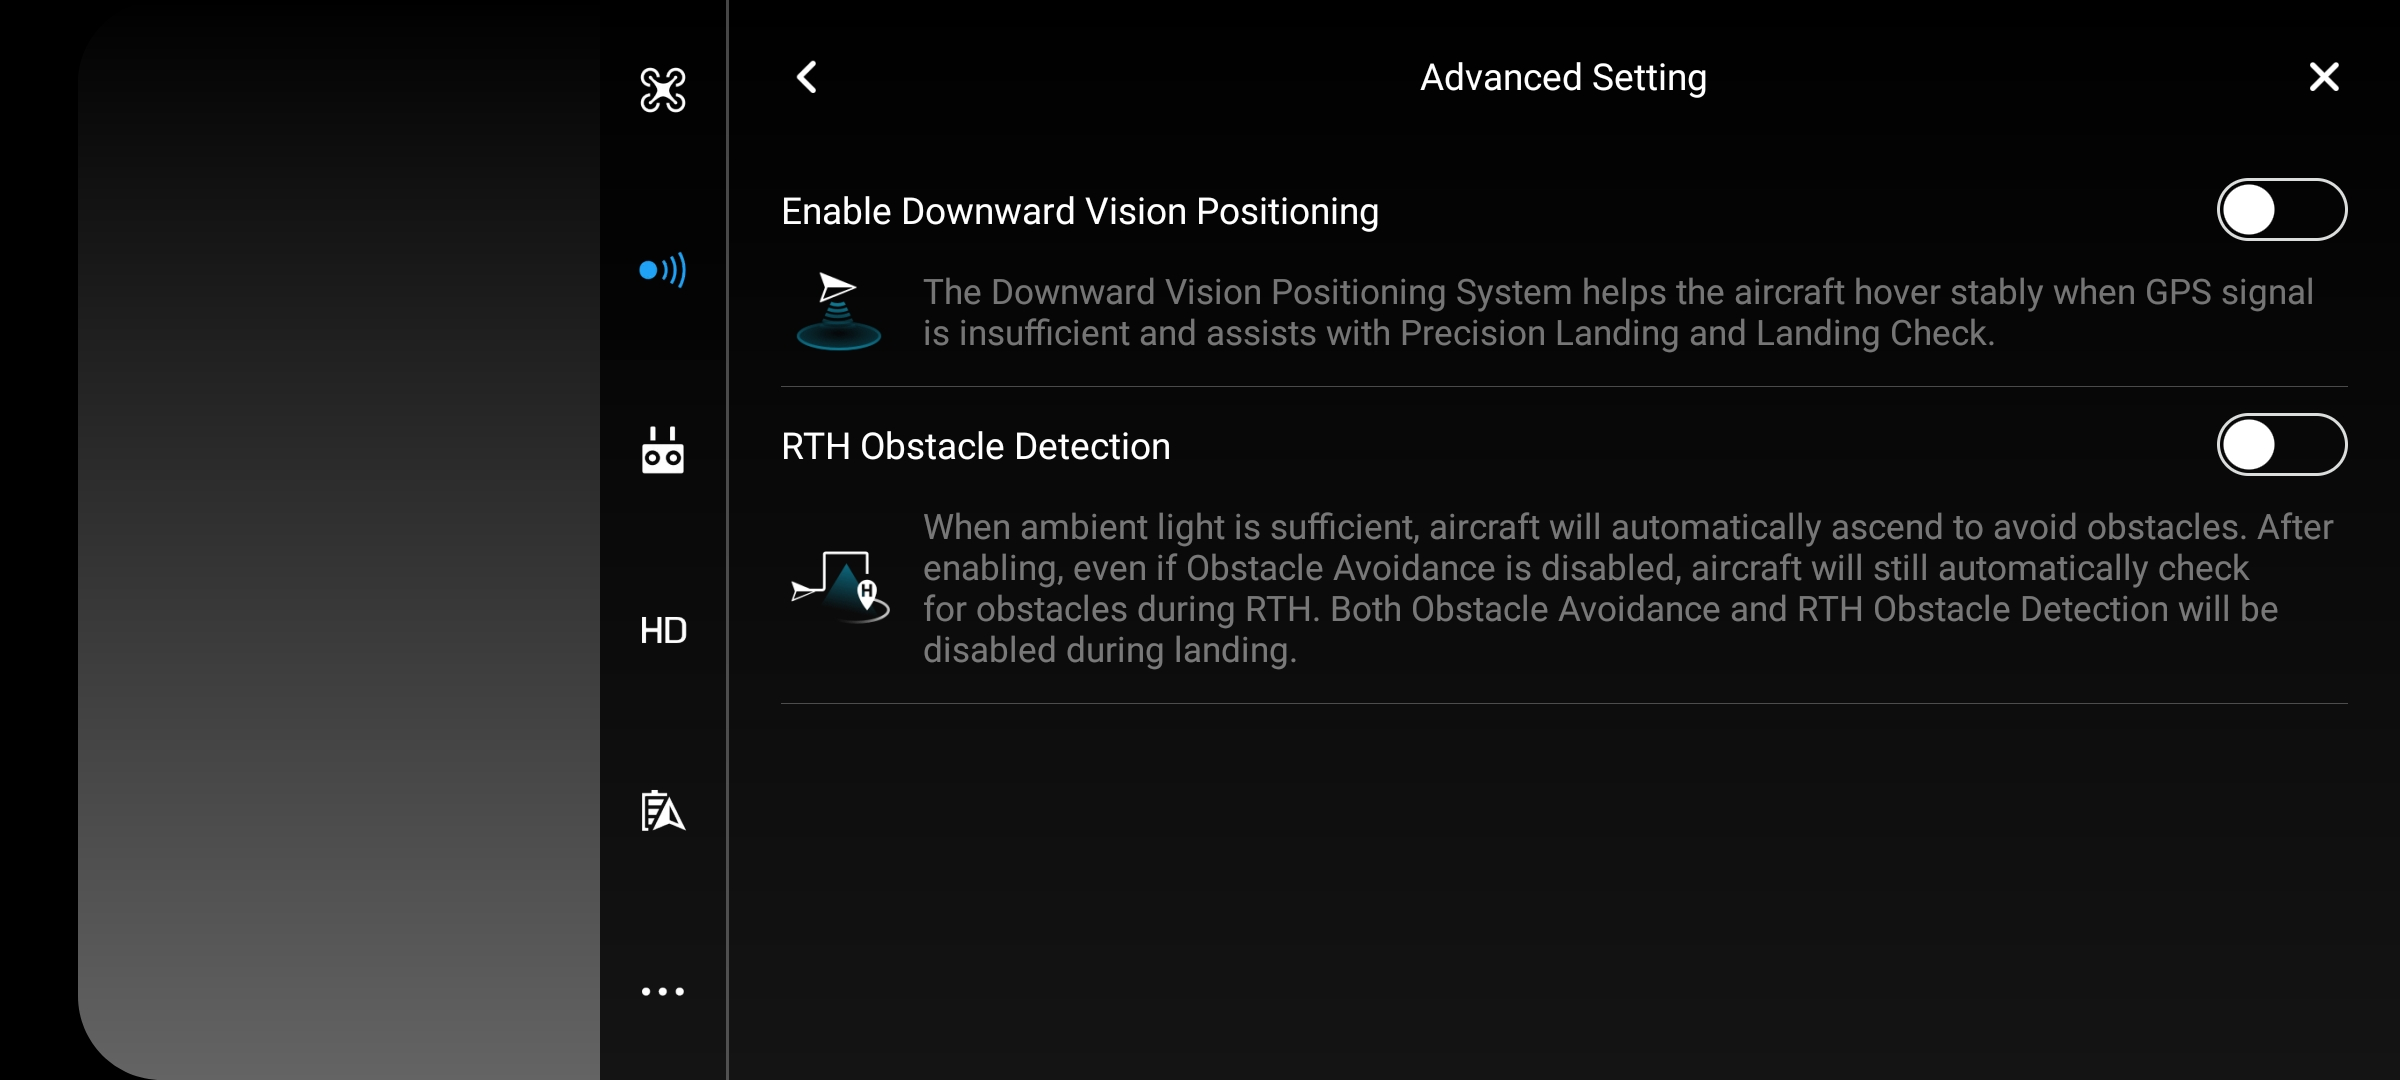
\includegraphics{images/VN/DJI-VN-AdvancedSettings.jpg}
\caption{Advanced Settings}
\end{figure}

The Advanced Settings for the Visual Navigation Settings allow for the enabling/disabling of both the Downward vision positioning system and the return-to-home obstacle detection feature.

\end{document}
